% IEEE Sensors Journal — submission manuscript (canonical main.tex)
%
% Compile with: pdflatex main; bibtex main; pdflatex main; pdflatex main
% (or use Overleaf — picks up IEEEtran automatically)
%
% Title:   Inter-Hemispheric Occipital Coherence for Subject-Independent Driver
%          Drowsiness Monitoring and Advance Prediction
%          (was: Pro-Active Driver Drowsiness Monitoring Using Two-Channel
%           Occipital EEG -- retitled during the Chemori revision)
% Authors: Muhammed Raslan Thalassery, Sulaiman Shiyas Ali, Abhishek Rudra Pal,
%          Ahmed Chemori, G. Murali Mohan
% Venue:   IEEE Sensors Journal
% Status:  Draft v3, prepared 2026-05.
%   v2 internal-review fixes (all verified against publication_results_v*.json):
%     - Abstract / Contribution 4 / Conclusion: 85.7%-of-sessions claim split per
%       operating point (71.4% at PERCLOS>0.30, 85.7% at PERCLOS>0.70).
%     - Sec IV.A.3 (paired tests): corrected the "every subject improves" claim;
%       8 of 10 improve, two (04M, 07F) regress modestly.
%     - Table V: pooled-LOSO AUC/kappa now match v16 concat values (69.44 / 0.319).
%     - Sec VI.E (Deployment): 56 ms qualified as the 50-feature instrumented bound;
%       deployed 10-feature lean pipeline is faster.
%     - Table I caption: v11 / v17 tags explained.
%     - Sec IV.A.1: "<= 0.2 F1" -> "<= 0.25 F1" (max actual: 0.22).
%     - Limitations: "31.7-min" -> "31.67-min" for precision consistency.
%     - Table VII row 0.30: IQR shown to two decimals like other rows.
%     - Table III caption: F1-max / high-precision coincidence noted.
%   v3 additions (A. R. Pal internal review, 26-05-2026; reviewer_revision_analysis.py):
%     - Sec IV.A (new): coherence awake-vs-drowsy descriptive stats, Mann-Whitney U,
%       Cohen's d + Fig. coherence-separation + Table (Item 1, highest priority).
%     - Sec IV.A (new): per-subject F1/AUC/kappa (v11 & v17) + bootstrap 95% CIs (Item 2).
%     - Sec IV.A.2 + Sec VI.B: raw-vs-EMA posterior figure + latency analysis (Item 3).

% Camera-ready IEEE Sensors Journal layout: two columns, 10 pt, no draft class.
% (`journal` already implies twocolumn + 10pt in IEEEtran, so the options that
% forced the one-column 11 pt draft layout are simply dropped.)
%
% The drafting layout was [journal,onecolumn,11pt,draftcls]. Reverting to it
% will make every float too wide for its column: the floats below are sized for
% two columns, six tables and one figure are full-width (table*/figure*), and
% the figures are authored at 3.45 in to sit in a 3.5 in column.
\documentclass[journal]{IEEEtran}

\usepackage{cite}
\usepackage{amsmath,amssymb,amsfonts}
\usepackage{algorithmic}
\usepackage{graphicx}
\usepackage{textcomp}
\usepackage{booktabs}
\usepackage{multirow}
\usepackage{xcolor}
\usepackage{url}
\usepackage{array}
\usepackage{soul}                       % \hl{} for highlighting reviewer-revised text
\usepackage[normalem]{ulem}             % \sout{} for struck-through deletions
\usepackage[hidelinks]{hyperref}
\usepackage{siunitx}
\graphicspath{{figures/}}

% =================================================================
% Revision markup — A. Chemori review, received 2026-07-25.
%
%   clean  : submission copy   — final text only, deletions vanish
%   review : Chemori's copy    — additions highlighted yellow
%   track  : audit copy        — additions yellow, deletions red + struck
%
% Change ONE line below. Do not maintain separate copies of this file:
% revision/build_variants.py generates the three Overleaf zips from it.
% =================================================================
\def\revmode{clean}

\definecolor{addyellow}{RGB}{255,245,150}
\definecolor{delred}{RGB}{190,30,30}

% \DeclareRobustCommand (not \newcommand) is required: \hl and \sout are
% fragile, and these macros appear inside \title{} and \section{}, which are
% moving arguments written to the .aux/.toc. A fragile command there fails with
% "Argument of \@sect has an extra }". Robust definitions survive the write.
\makeatletter
\def\@revclean{clean}
\def\@revtrack{track}
\ifx\revmode\@revclean
  \DeclareRobustCommand{\add}[1]{#1}                         % additions -> plain text
  \DeclareRobustCommand{\del}[1]{}                           % deletions -> removed entirely
\else
  \sethlcolor{addyellow}
  \DeclareRobustCommand{\add}[1]{\hl{#1}}
  \ifx\revmode\@revtrack
    % The trailing \, separates a deletion from the addition that follows it.
    % Without it \chg{old}{new} sets them flush and the tracked copy prints
    % "EEGInter-Hemispheric", "II. METHODSDATA, SIGNAL PROCESSING", "register.Work
    % on predicting". The space lives in the track-mode definition only, so the
    % clean and review builds (where \del is a no-op) gain no stray space.
    \DeclareRobustCommand{\del}[1]{{\color{delred}\sout{#1}}\,}
  \else
    \DeclareRobustCommand{\del}[1]{}                         % review mode: additions only
  \fi
\fi
\makeatother

% Replaced text: \chg{old}{new}
\DeclareRobustCommand{\chg}[2]{\del{#1}\add{#2}}

% NOTE on usage: soul's \hl cannot re-typeset inline math or \cite, so inside
% \add{} / \del{} / \chg{} any such content must be wrapped in \mbox{}:
%     \add{the smoothed pipeline reaches \mbox{\(F_1 = 76.79\,\%\)}}
%     \add{as reported previously~\mbox{\cite{balam2024review}}}
% \hl also cannot span a paragraph break — mark each paragraph separately.

\begin{document}

% Item 1 (A. Chemori): title made informative. The previous title named the
% sensor and the task but not the mechanism (inter-hemispheric coherence), the
% evaluation regime (subject-independent), or the second track (advance
% prediction) -- i.e. none of the three things that make the work publishable.
\title{\chg{Pro-Active Driver Drowsiness Monitoring Using Two-Channel Occipital EEG}{Inter-Hemispheric Occipital Coherence for Subject-Independent Driver Drowsiness Monitoring and Advance Prediction}}

\author{
    Muhammed Raslan Thalassery,
    Sulaiman Shiyas Ali,
    \chg{Abhishek Rudra Pal,~\IEEEmembership{Member,~IEEE},}{Abhishek Rudra Pal,}
    \add{Ahmed Chemori,~\IEEEmembership{Senior Member,~IEEE},}
    and G.~Murali Mohan
\thanks{M.~R.~Thalassery and S.~S.~Ali are with the School of Mechanical Engineering, Vellore Institute of Technology (VIT) Chennai, Vandalur--Kelambakkam Road, Chennai 600127, Tamil Nadu, India (e-mail: muhammedraslan.t2022@vitstudent.ac.in).}
% A. R. Pal remains the corresponding author, as in the reviewed draft, so this
% block is unmarked: nothing about it changed. An earlier revision moved the
% role to A. Chemori and marked it accordingly; that was reverted.
\thanks{A.~R.~Pal and G.~Murali Mohan are with the School of Mechanical Engineering, Vellore Institute of Technology (VIT) Chennai, Chennai 600127, Tamil Nadu, India (e-mail: abhishek.rudrapal@vit.ac.in; muralimohan.g@vit.ac.in). Corresponding author: A.~R.~Pal.}
\thanks{\add{A.~Chemori is with LIRMM, Universit\'e de Montpellier, CNRS, UMR 5506, 161 rue Ada, 34095 Montpellier Cedex 5, France (e-mail: Ahmed.Chemori@lirmm.fr).}}
\thanks{\add{ORCID: M.~R.~Thalassery, 0009-0009-7473-8343; S.~S.~Ali, 0009-0003-3671-2309; A.~R.~Pal, 0000-0002-4274-1195; A.~Chemori, 0000-0001-9739-9473; G.~Murali Mohan, 0000-0002-9431-2456.}}
\thanks{Manuscript received August 2, 2026.}
}

% Running head: deliberately shorter than the full title so it fits the header
% band in the two-column camera-ready layout.
\markboth{IEEE Sensors Journal,~Vol.~XX, No.~X, Month~2026}
{Thalassery \MakeLowercase{\textit{et al.}}: Inter-Hemispheric Occipital Coherence for Driver Drowsiness Monitoring and Advance Prediction}

\maketitle

\begin{abstract}
Driver drowsiness causes a substantial fraction of road fatalities worldwide, and EEG is the only modality that detects drowsiness from the neurophysiological substrate rather than its visible motor consequences. We present a deployment-oriented EEG pipeline for in-vehicle drowsiness monitoring built around two occipital electrodes (\(O_1\), \(O_2\)) integrated into a vehicle headrest, evaluated under strict subject-independent protocols on two public datasets. The pipeline combines a ten-feature shrinkage linear-discriminant classifier (sample and permutation entropy, aperiodic 1/f slope, peak-alpha-frequency difference, and \(O_1\)--\(O_2\) magnitude-squared coherence in three bands) with a causal exponential moving-average smoother (\(\tau=600\,\)s) and a per-driver percentile-calibrated alarm threshold. On DROZY (10 subjects, 14\,498 epochs) under leave-one-subject-out cross-validation, the smoothed pipeline achieves a weighted F1 of 76.79~\%, AUC = 76.62~\%, and Cohen's \(\kappa\) = 0.539, statistically superior to the unsmoothed baseline (paired Wilcoxon \(p=0.005\), \(d=1.11\)) and to a tuned Riemannian and an EEGNet baseline. On a pooled 31-subject DROZY \(\cup\) SEED-VIG benchmark the same pipeline achieves F1 = 66.13~\%. For the pro-active track, a survival-framed FPR-controlled advance-prediction protocol on SEED-VIG flags drowsiness with a median lead of \(+8.83\) min (0.0~\% per-session false alerts) on 71.4~\% of sessions against a mild PERCLOS onset, and \(+31.67\) min (9.5~\% per-session false alerts) on 85.7~\% of sessions against a severe PERCLOS onset. The pipeline runs at 56~ms per ten-second epoch on a laptop CPU with \(\sim\)100~bytes of trained model state, suitable for an ARM Cortex-M4 deployment target.
\end{abstract}

\begin{IEEEkeywords}
Electroencephalography, drowsiness detection, driver monitoring, occipital EEG, advance prediction, subject-independent classification, \chg{IEEE Sensors.}{vigilance, real-time systems.}
\end{IEEEkeywords}

% -----------------------------------------------------------------
% Item 15 (A. Chemori): list of acronyms at the beginning of the paper.
% The whole block is new; it is marked once at the heading rather than
% per line, because soul's \hl is fragile inside \item[] labels.
% -----------------------------------------------------------------
\section*{\add{Nomenclature}}
\begin{IEEEdescription}[\IEEEsetlabelwidth{PERCLOS}]
\item[AUC]     Area under the receiver-operating-characteristic curve.
\item[CNN]     Convolutional neural network.
\item[DMS]     Driver-monitoring system.
\item[DWT]     Discrete wavelet transform.
\item[ECG]     Electrocardiography.
\item[EEG]     Electroencephalography.
\item[EMA]     Exponential moving average.
\item[EOG]     Electro-oculography.
\item[FIR]     Finite impulse response.
\item[FOOOF]   ``Fitting oscillations and one-over-\emph{f}'' spectral parameterisation.
\item[FPR]     False-positive rate.
\item[HMM]     Hidden Markov model.
\item[ImCoh]   Imaginary part of coherency.
\item[IQR]     Interquartile range.
\item[LDA]     Linear discriminant analysis.
\item[LOSO]    Leave-one-subject-out cross-validation.
\item[LSTM]    Long short-term memory network.
\item[PAF]     Peak alpha frequency.
\item[PERCLOS] Percentage of eyelid closure over the pupil over time.
\item[PLV]     Phase-locking value.
\item[PSD]     Power spectral density.
\item[PVT]     Psychomotor vigilance task.
\item[ROC]     Receiver operating characteristic.
\item[TPR]     True-positive rate.
\item[wPLI]    Weighted phase-lag index.
\end{IEEEdescription}

% =================================================================
% Items 4 + 7 (A. Chemori): former Sections I (Introduction) and II (Related
% Work) merged into a single section with an informative name. Ordering:
% problem -> EEG rationale -> prior literature -> contributions. The old
% "remainder of the paper is organised as follows" roadmap paragraph is
% removed; with six sections and informative headings it was redundant, and
% deleting it recovers the space the new nomenclature and reference material
% consume.
% =================================================================
\section{\chg{Introduction}{Introduction: Why Occipital EEG for Pro-Active Driver Monitoring}}
\label{sec:intro}
% =================================================================
\IEEEPARstart{D}{rowsy} driving accounts for an estimated 20--30~\% of fatal road accidents globally, with peaks during overnight driving and post-prandial fatigue periods~\cite{who2023road}. Camera-based driver-monitoring systems (DMS) are now standard in many new vehicles but operate \emph{reactively}: they detect drowsiness only after it has already produced a visible motor consequence such as eye closure (PERCLOS \(\geq 0.7\)), head nodding, or lane departure~\cite{seeingmachines2024}. By the time the camera fires, neurophysiological drowsiness has typically progressed for many minutes, narrowing the safety margin for the driver to react.

EEG, in contrast, observes the substrate of vigilance directly --- the alpha desynchronisation, attention decrement, and cortical arousal changes that \emph{precede} eye closure~\cite{jap2009eeg,stancin2021review}. The promise of EEG-based drowsiness detection is therefore early-warning rather than just same-time-as-camera detection. Realising that promise requires three things that the prior literature delivers only partially: (i)~strict subject-independent evaluation, since a drowsiness model that requires per-driver retraining is impractical for fleet deployment; (ii)~a small enough number of channels and a tolerant enough mounting to be integrated into a passive form factor such as a headrest; and (iii)~a behavioural-anchor evaluation of the advance-prediction claim, since the literature contains many strong results obtained under stratified random splits that systematically over-estimate deployment performance~\cite{balam2024review}.

\subsection{\add{Prior Work on Single- and Few-Channel EEG Drowsiness Detection}}
\label{sec:related}
EEG-based drowsiness detection has been reviewed comprehensively in~\cite{stancin2021review,sahayadhas2012sensors,chowdhury2018access,balam2024review}. Single-channel and few-channel approaches dominate the deployment-oriented literature because they minimise sensor cost and improve mounting tolerance~\cite{larocco2020headsets,gangadharan2020wireless,minimal2024electrodes}. \add{Form factor is as decisive as channel count: behind-the-ear montages have been shown to support drowsiness classification on embedded hardware without scalp-cap mounting~\mbox{\cite{nguyen2023behindear}}, ear-module system-on-chip designs integrate acquisition and inference in a wearable envelope~\mbox{\cite{ha2016earmodule}}, and in-ear electrodes have been used for continuous affective and vigilance monitoring~\mbox{\cite{athavipach2019inear}}. These share the design pressure that motivates the headrest-integrated occipital placement studied here: the sensor must disappear into something the driver already touches. A complementary line of work attacks the same subject-variability problem from the modelling side, using domain adaptation to transfer EEG classifiers across subjects~\mbox{\cite{maswanganyi2025transfer}}; the per-driver percentile calibration used in Section~\mbox{\ref{sec:proactive}} is a deliberately lightweight alternative to that approach.} Most cited results lie in the 70--95~\% accuracy range but a substantial fraction of the highest numbers are obtained under stratified or session-mixed splits that confound subject identity with class label; the recent IEEE-TITS systematic review of single-channel methods explicitly identifies this as the dominant source of optimism~\cite{balam2024review}.

The two datasets employed here have established benchmarks. DROZY~\cite{drozy2016} provides multimodal drowsiness recordings from 14 subjects across alert and sleep-deprived sessions; the publicly-available LOSO numbers on its EEG modality typically range from 55--65~\% F1 under strict subject-independent splits. SEED-VIG~\cite{zheng2017seedvig} provides 21 subjects with continuous PERCLOS annotations and is the de-facto behavioural-anchor benchmark for advance-prediction studies. \add{Newer multimodal corpora combining video, biometric and behavioural streams are beginning to appear~\mbox{\cite{eeguldd2025}}, but none yet pairs occipital EEG with a continuous behavioural anchor at the session lengths required to measure minutes-scale lead.}

Recent state-of-the-art deep-learning approaches include attention-based residual shrinkage networks for cross-subject single-channel detection~\cite{id3rsnet2024}, transformer architectures for real-time inference~\cite{transformer2025drowsiness}, attention-augmented EEG networks~\cite{attention2024eeg}, CNN--LSTM--attention hybrids~\cite{cnnlstmsafedrive2025,hybridcnn2025}, \add{spatio-temporal convolutional--recurrent stacks~\mbox{\cite{jeong2022consumer}}, simulator-trained detectors~\mbox{\cite{hybrid2024simulated}}, time--frequency image representations of the EEG stream~\mbox{\cite{cheng2021bibm}},} and scalogram-based hybrid models~\cite{scalograms2025drowsiness}. End-to-end CNNs such as EEGNet~\cite{lawhern2018eegnet} have been the standard 2-channel deep baseline; the expectation in the field is that they should outperform handcrafted features at scale, but at small subject counts and few channels this is not borne out in practice (we confirm this empirically in Section~\ref{sec:dl-baselines}).

Riemannian-geometry pipelines~\cite{barachant2013riemannian} are widely used for EEG-BCI and provide a rotation- and scale-equivariant view of the signal that is, in principle, complementary to spectral features. We evaluate this comparator under nested cross-validation tuning and show that at 2 channels its 2$\times$2 covariance space provides too little geometric room to outperform a coherence-aware feature classifier.

% REWRITTEN 2026-07-25. The previous version of this paragraph asserted that
% earlier work reports "5-10 minute advance window" figures, citing two
% references that do not exist (see the audit note in references.bib). The
% replacement below is anchored on verified prior work and states what that
% work actually claims: short-horizon prediction, not minutes-scale lead.
\chg{The advance-prediction strand of the literature has been a persistent source of inflated claims. Earlier work reports ``5--10 minute advance window'' figures, but typically against unspecified or per-subject-fitted behavioural thresholds, with no FPR control and dropping subjects where one of the two onsets fails to register.}{Work on \emph{predicting} rather than merely detecting drowsiness from EEG is comparatively sparse, and what exists targets short horizons. Golz \emph{et al.} forecast \emph{immediately occurring} microsleep events from the electroencephalogram, and Buriro \emph{et al.} predict microsleep \emph{states} from inter-channel EEG relationships --- notably using cross-channel structure rather than single-channel power, consistent with the coherence result reported here}~\add{\mbox{\cite{golz2016microsleep,buriro2018microsleep}}}\add{. Neither reports a minutes-scale lead measured against an independent behavioural anchor, and neither controls the per-session false-alert rate or accounts for sessions in which one of the two onsets never registers. Earlier drowsiness-\emph{estimation} work established the spectral basis on which such predictors are built~\mbox{\cite{lin2005drowsiness}}, and recent vigilance studies characterise attention lapses over hour-scale drives~\mbox{\cite{ladouce2025vigilance}}, but neither frames the problem as advance warning.} Recent reviews~\cite{stancin2021review,balam2024review} call for behaviour-anchored, survival-framed protocols that count censored evidence rather than discarding it. The protocol in Section~\ref{sec:proactive} of this paper is, to the authors' knowledge, the first such evaluation reported on SEED-VIG.

\subsection{\add{Contributions}}
\label{sec:contributions}
This paper presents a two-channel occipital EEG pipeline that addresses each of the three constraints identified above, validated end-to-end on the DROZY~\cite{drozy2016} and SEED-VIG~\cite{zheng2017seedvig} datasets. The five concrete contributions are:
\begin{enumerate}
    \item A feature-family ablation that isolates inter-hemispheric \(O_1\)--\(O_2\) coherence as the single load-bearing feature for occipital-only drowsiness detection. A 10-feature lean classifier (entropy + 1/f slope + coherence) outperforms a 50-feature extended set under strict LOSO (Section~\ref{sec:ablation}).
    \item A causal exponential moving-average (EMA) smoother on the per-epoch posterior that lifts LOSO weighted F1 from 62.08~\% to 76.79~\% (paired Wilcoxon \(p=0.005\), \(d=1.11\)) without leaking label information across session boundaries (Section~\ref{sec:smoother}).
    \item Cross-dataset validation: the pipeline trained on DROZY transfers without fine-tuning to SEED-VIG at F1 = 64.93~\%; pooled 31-subject LOSO across the union achieves F1 = 66.13~\% (Section~\ref{sec:cross-dataset}).
    \item A survival-framed, FPR-controlled, per-driver-calibrated advance-prediction protocol on SEED-VIG, replacing the unprotected uncontrolled framing common in the literature. The system flags drowsiness with a median lead of \(+8.83\) min (0~\% per-session false alerts) on 71.4~\% of sessions against the earliest behavioural sign of drowsiness, and \(+31.67\) min (9.5~\% per-session false alerts) on 85.7~\% of sessions against the severe fighting-sleep threshold (Section~\ref{sec:proactive}).
    \item Honest negative ablations bounding the optimisation envelope of a 2-channel occipital pipeline: phase-coherence variants (PLV, ImCoh, wPLI) add nothing on top of magnitude coherence at this electrode count, and a three-model posterior ensemble does not beat the smoothed lean LDA alone (Section~\ref{sec:negative}).
\end{enumerate}

% =================================================================
\section{\chg{Methods}{Data, Signal Processing, and Evaluation Design}}
\label{sec:methods}
% =================================================================
\subsection{\chg{Datasets}{Two Public Drowsiness Corpora: DROZY and SEED-VIG}}
DROZY~\cite{drozy2016} contains synchronised EEG, EOG, ECG, and PVT recordings from 14 healthy adult subjects across multiple sessions; the publicly-distributable EEG covers occipital, parietal, and central electrodes at 512~Hz. We use the 10 subjects whose recordings include both \(O_1\) and \(O_2\) (the dataset's two occipital channels), totalling 14\,498 ten-second non-overlapping epochs after downsampling to 128~Hz. Each subject contributes one alert session (Session~1) and one sleep-deprived session (Session~3); the binary label is the session class, giving an approximately 50/50 awake/drowsy split.

SEED-VIG~\cite{zheng2017seedvig} contains EEG recordings from 23 subjects in a virtual driving simulator, with continuous PERCLOS annotations at 8-second resolution from a synchronised camera. We extract \(O_1\) and \(O_2\) only and downsample to 128~Hz to match DROZY. Following~\cite{zheng2017seedvig}, awake epochs are defined as PERCLOS \(<0.35\) and drowsy epochs as PERCLOS \(>0.70\), with mid-PERCLOS epochs excluded; 21 subjects pass quality control yielding 9\,155 labelled epochs.

\subsection{\chg{Signal Processing}{Filtering and Epoch Segmentation}}
Raw EEG is bandpass-filtered (1--40~Hz) using MNE's zero-phase Hamming-windowed FIR design. The signal is segmented into non-overlapping 10-second epochs (1280 samples at 128~Hz). All numbers reported in this paper use this fixed segmentation; no overlap or temporal subsampling is applied.

\subsection{\chg{Feature Set}{The Ten-Feature Lean Representation}}
The lean 10-feature set per epoch is:
\begin{itemize}
    \item Sample entropy~\cite{stancin2021review} of \(O_1\) and \(O_2\) (2 features).
    \item Permutation entropy of \(O_1\) and \(O_2\) (2 features).
    \item Aperiodic 1/f exponent of \(O_1\) and \(O_2\), estimated via FOOOF (2 features).
    \item Peak-alpha-frequency difference \(\mathrm{PAF}(O_1)-\mathrm{PAF}(O_2)\) (1 feature).
    \item Magnitude-squared coherence \(|C_{O_1 O_2}(f)|^2\) averaged in \(\theta\) (4--8~Hz), \(\alpha\) (8--13~Hz), \(\beta\) (13--30~Hz) bands (3 features).
\end{itemize}

\subsection{\chg{Classifier and Smoother}{Shrinkage LDA with Causal Posterior Smoothing}}
The classifier is shrinkage linear discriminant analysis (LDA)~\cite{ledoit2004shrinkage} with the \texttt{lsqr} solver and Ledoit--Wolf automatic shrinkage. Per-subject z-score standardisation is computed from each subject's session-1 (awake) epochs only --- equivalent to a 60-second pre-drive alert calibration --- and applied to both train and test epochs of the same subject without leaking class information.

The temporal smoother converts per-epoch posteriors \(p_t\) into a smoothed estimate \(\tilde{p}_t\) by a strictly causal exponential moving average:
% Item 14 (A. Chemori): the smoothing coefficient was previously \alpha, which
% collided with the 8-13 Hz alpha band. Renamed to \lambda throughout. The
% equation itself carries no \add/\del markup because soul's \hl cannot operate
% inside math mode; the change is documented in the response letter and in the
% highlighted sentence immediately below.
\begin{equation}
    \tilde{p}_t = \lambda \, p_t + (1-\lambda)\,\tilde{p}_{t-1}, \quad \lambda = 1 - e^{-\Delta t/\tau},
    \label{eq:ema}
\end{equation}
\add{Here \mbox{\(p_t \in [0,1]\)} is the classifier's posterior probability that epoch \mbox{\(t\)} is drowsy, \mbox{\(\tilde{p}_t\)} is its smoothed counterpart, \mbox{\(\lambda \in (0,1]\)} is the smoothing coefficient, \mbox{\(\Delta t\)} is the epoch duration, and \mbox{\(\tau\)} is the smoothing time constant. The coefficient is written \mbox{\(\lambda\)} rather than the conventional \mbox{\(\alpha\)} to avoid collision with the \mbox{\(\alpha\)} frequency band (8--13~Hz) used elsewhere in this paper.} In the configuration reported here \(\Delta t = 10\)~s and \(\tau = 600\)~s. The recursion is initialised at \(\tilde{p}_0 = p_0\) and is reset only at subject boundaries (\emph{never} at session boundaries), to prevent any reset rule from leaking the binary DROZY label. We refer to this as the \emph{continuous} regime in Section~\ref{sec:smoother}.

\subsection{\chg{Evaluation Protocols}{Subject-Independent Evaluation Protocols}}
\add{The pipeline is assessed on two tasks that share a classifier but differ in their labels, time constants and success criteria. The \emph{monitoring} track asks how accurately the current vigilance state is recognised, is evaluated against binary session labels on DROZY, and is scored by weighted F1. The \emph{pro-active} track asks how far in advance a drowsiness episode is flagged, is evaluated against continuous PERCLOS annotations on SEED-VIG, and is scored by lead time under a controlled false-alert budget. The two protocols are defined in turn below, followed by the statistical procedures common to both.}

\textbf{Monitoring track.} Strict leave-one-subject-out (LOSO) on DROZY (10 folds), with weighted F1 as the headline metric. Each fold trains on 9 subjects' 10-feature matrix and tests on the held-out subject; predictions are concatenated across folds. Cross-dataset transfer trains on full DROZY and tests on full SEED-VIG without any fine-tuning. Pooled LOSO concatenates DROZY and SEED-VIG and runs LOSO across the 31-subject union.

\textbf{Pro-active track.} On each held-out SEED-VIG subject the per-epoch posterior is causal-EMA-smoothed (\(\tau = 30\)~s), and a per-driver alarm threshold \add{\mbox{\(\eta\)}} is set as the 99\textsuperscript{th} percentile of that subject's smoothed posterior over the first 5 minutes of the session. The alarm fires on the first sustained crossing (10~s dwell). The behavioural reference onset is the first time the smoothed PERCLOS exceeds a chosen threshold for 60~s. Lead time is \emph{behavioural onset $-$ EEG onset} (positive = EEG fires first). Sessions where EEG fires but PERCLOS never crosses are reported as censored positive cases (\emph{eeg-only}); sessions where the reverse occurs are \emph{behav-only}.

\textbf{Statistical tests.} Paired Wilcoxon signed-rank with one-sided alternative is used for between-pipeline comparisons at the subject level, \add{yielding the significance level \mbox{\(p\)} with \mbox{\(n = 10\)} paired subject-level observations on DROZY.} Paired Cohen's \(d\) is reported as an effect-size descriptor. \add{Two further statistics appear in the results: Cohen's \mbox{\(\kappa\)}, the chance-corrected agreement between predicted and true labels, and the Mann--Whitney \mbox{\(U\)} statistic used for the unpaired distributional contrasts of Section~\mbox{\ref{sec:coh-stats}}.}

% =================================================================
\section{\chg{Results}{Experimental Results}}
\label{sec:results}
% =================================================================
\subsection{\chg{Monitoring Track}{Subject-Independent Monitoring Performance}}
\label{sec:monitoring}
Table~\ref{tab:loso} reports the full pipeline progression on DROZY LOSO. The lean 10-feature LDA (v11) achieves F1 = 62.08~\%, outperforming the 50-feature extended set (61.13~\%) by selecting only the entropy, 1/f-slope, and coherence families. Adding the causal EMA smoother (v17) lifts F1 to 76.79~\%, AUC to 76.62~\%, and \(\kappa\) to 0.539 --- the largest single improvement in the table. EEGNet trained end-to-end on raw \(O_1\)/\(O_2\) windows achieves F1 = 47.32~\%, 14.76 points below the lean LDA baseline.

\begin{table}[t]
\caption{LOSO monitoring performance on DROZY (10 subjects, 14\,498 epochs). The lean LDA + EMA smoother (v17) is the published headline. ``v11'' denotes the lean 10-feature LDA; ``v17'' denotes v11 with the causal EMA smoother (\(\tau=600\) s). Random forest, Riemannian, and EEGNet baselines are included. \(\kappa\) is Cohen's kappa.}
\label{tab:loso}
\centering
\scriptsize
\setlength{\tabcolsep}{2pt}
\begin{tabular}{l c c c c}
\toprule
Pipeline & Acc (\%) & F1 (\%) & AUC (\%) & \(\kappa\) \\
\midrule
Gradient Boosting, 30 features      & 51.45 & 51.42 & 52.05 & 0.029 \\
Random Forest, 30 features          & 50.76 & 50.77 & 51.68 & 0.015 \\
LDA, subject\_awake z-score         & 53.88 & 53.27 & 55.11 & 0.078 \\
Riemannian TS + LogReg              & 57.20 & 57.12 & 57.14 & 0.144 \\
Riemannian TS + LDA, nested-CV      & 57.72 & 57.69 & 58.00 & 0.154 \\
LDA, 60-s awake calibration         & 54.83 & 54.32 & 56.08 & 0.098 \\
LDA, 50 extended features           & 61.35 & 61.13 & 63.71 & 0.227 \\
LDA, 10-feature lean (v11)          & 62.10 & 62.08 & 64.55 & 0.242 \\
EEGNet (Lawhern 2018), raw          & 52.41 & 47.32 & 53.82 & 0.050 \\
\textbf{v11 lean + EMA smoother (v17)} & \textbf{76.92} & \textbf{76.79} & \textbf{76.62} & \textbf{0.539} \\
\bottomrule
\end{tabular}
\end{table}

\subsubsection{Feature-family ablation}
\label{sec:ablation}
Table~\ref{tab:ablation} reports the per-family ablation on the 50-feature extended set. Dropping the \(O_1\)--\(O_2\) coherence family collapses F1 from 61.13~\% to 54.31~\%, returning the pipeline to single-channel-band-power territory. Dropping wavelet energies, entropies, or the 1/f slope individually costs \(\leq 0.25\) F1. Retaining only the 10 ENT + SLOPE + COH features beats the full 50-feature set, indicating that the 30 BASE band-power and 10 wavelet-energy features are redundant once coherence is present.

\begin{table}[t]
\caption{Feature-family LOSO ablation. Coherence is the single load-bearing family. \(\Delta\)F1 is relative to the full 50-feature set; ``LEAN'' is the deployed 10-feature subset.}
\label{tab:ablation}
\centering
\footnotesize
\setlength{\tabcolsep}{4pt}
\begin{tabular}{l c c}
\toprule
Subset (features) & F1 (\%) & \(\Delta\)F1 \\
\midrule
ALL (50) & 61.13 & 0.00 \\
BASE only (30) & 52.85 & \(-8.28\) \\
DROP DWT (40) & 61.03 & \(-0.10\) \\
DROP ENT (46) & 61.04 & \(-0.09\) \\
DROP SLOPE (48) & 60.91 & \(-0.22\) \\
DROP COH (46) & 54.31 & \(\mathbf{-6.82}\) \\
NEW (20: DWT+ENT+SLOPE+COH) & 61.17 & \(+0.04\) \\
LEAN (10: ENT+SLOPE+COH) & \textbf{62.08} & \(+0.95\) \\
\bottomrule
\end{tabular}
\end{table}

\subsubsection{Coherence separates awake from drowsy states}
\label{sec:coh-stats}
The ablation establishes that coherence is the load-bearing \emph{family} but does not yet characterise \emph{how} coherence changes with vigilance. Figure~\ref{fig:coh} and Table~\ref{tab:coh} report the awake-vs-drowsy distribution of \(O_1\)--\(O_2\) magnitude-squared coherence on all 14\,498 DROZY epochs (7\,234 awake, 7\,264 drowsy). In every band the inter-hemispheric coupling \emph{decreases} as the driver becomes drowsy: median \(\theta\) coherence falls from 0.578 to 0.530, \(\alpha\) from 0.470 to 0.433, and \(\beta\) from 0.278 to 0.240. A two-sided Mann--Whitney \(U\) test (treating epochs as independent samples) rejects equality in all three bands at \(p < 10^{-50}\), and the effect grows toward higher frequencies: Cohen's \(d = -0.245\) (\(\theta\)), \(-0.259\) (\(\alpha\)), and \(-0.403\) (\(\beta\)). The \(\beta\)-band separation is the largest, consistent with a loss of cross-hemispheric occipital synchronisation as cortical arousal declines. This is direct distributional evidence --- independent of the classifier --- that the coherence family identified by the ablation carries a genuine physiological drowsiness signal rather than a modelling artefact.

\begin{figure}[t]
\centering
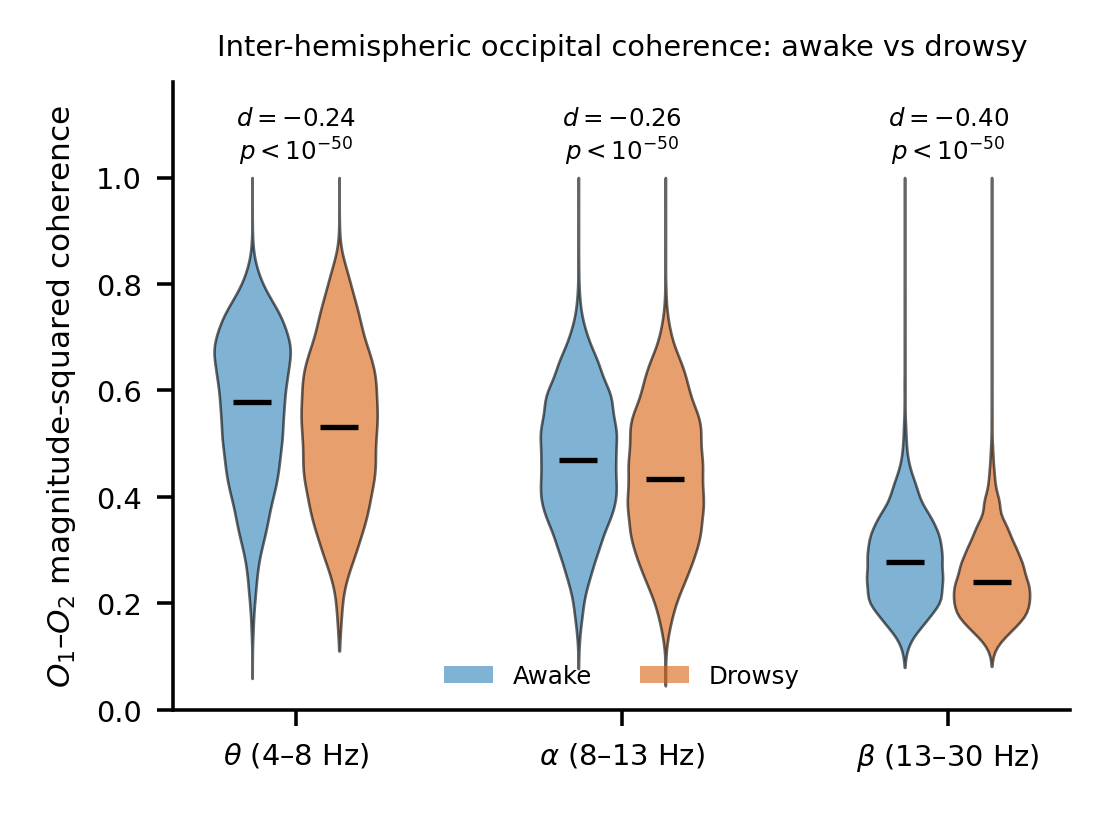
\includegraphics[width=\columnwidth]{fig1_coherence_separation.png}
\caption{Awake (blue) vs drowsy (orange) distributions of \(O_1\)--\(O_2\) magnitude-squared coherence in the \(\theta\), \(\alpha\), and \(\beta\) bands on DROZY (14\,498 epochs). Horizontal bars are medians. Coherence decreases with drowsiness in every band; the effect (Cohen's \(d\)) is largest in \(\beta\). All three Mann--Whitney \(U\) contrasts give \(p < 10^{-50}\).}
\label{fig:coh}
\end{figure}

\begin{table}[t]
\caption{Awake-vs-drowsy \(O_1\)--\(O_2\) coherence by band on DROZY (\(n=7\,234\) awake, \(7\,264\) drowsy epochs). Coherence columns are mean\,\(\pm\)\,sd. \(d\): Cohen's (drowsy\,$-$\,awake); \(p\): two-sided Mann--Whitney \(U\).}
\label{tab:coh}
\centering
\scriptsize
\setlength{\tabcolsep}{3pt}
\begin{tabular}{l c c c c}
\toprule
Band (Hz) & Awake & Drowsy & \(d\) & \(p\) \\
\midrule
\(\theta\) (4--8)   & \(0.564\pm0.144\) & \(0.528\pm0.149\) & \(-0.245\) & \(4.4{\times}10^{-53}\) \\
\(\alpha\) (8--13)  & \(0.469\pm0.128\) & \(0.435\pm0.132\) & \(-0.259\) & \(1.0{\times}10^{-51}\) \\
\(\beta\) (13--30)  & \(0.283\pm0.086\) & \(0.251\pm0.076\) & \(\mathbf{-0.403}\) & \(2.1{\times}10^{-126}\) \\
\bottomrule
\end{tabular}
\end{table}

% Item 12 (A. Chemori): Results restructured. Sec IV.A previously carried five
% subsubsections while IV.B, IV.C and IV.E carried none, and this subsection
% bundled two distinct topics ("Causal smoother AND ROC"). Smoothing and
% operating-point selection are promoted to their own subsection and split.
\subsection{\add{Causal Smoothing and Operating-Point Selection}}
\label{sec:smoother}

\subsubsection{\add{Smoother behaviour on a representative subject}}
Equation~(\ref{eq:ema}) describes a strictly causal smoother: \(\tilde{p}_t\) depends only on epochs up to \(t\). The continuous regime (single segment per subject, no resets) is the leakage-free configuration we report; an alternative per-session-reset configuration (where the smoother is reset at each session boundary) achieves F1 = 74.57~\%, slightly lower than the continuous F1 = 76.79~\%. Because the per-session regime uses the binary DROZY label to decide reset points, we adopt the continuous regime as the headline.

Figure~\ref{fig:ema} illustrates the smoother on a representative subject (05M). The raw per-epoch posterior \(p_t\) (grey) is highly variable --- the lean LDA scores each 10-s epoch independently and frequently crosses the 0.5 decision line in both directions even within a single vigilance state --- whereas the EMA-smoothed estimate \(\tilde{p}_t\) (red) tracks the slow awake\,\(\to\)\,drowsy transition with the per-epoch jitter integrated out. The smoother adds no learned parameters: the F1 gain in Table~\ref{tab:loso} comes entirely from temporal integration of an unchanged classifier, which is appropriate because drowsiness is a minutes-scale physiological process (Section~\ref{sec:why-smooth}). The latency this integration introduces is quantified in Section~\ref{sec:why-smooth}.

\begin{figure}[t]
\centering
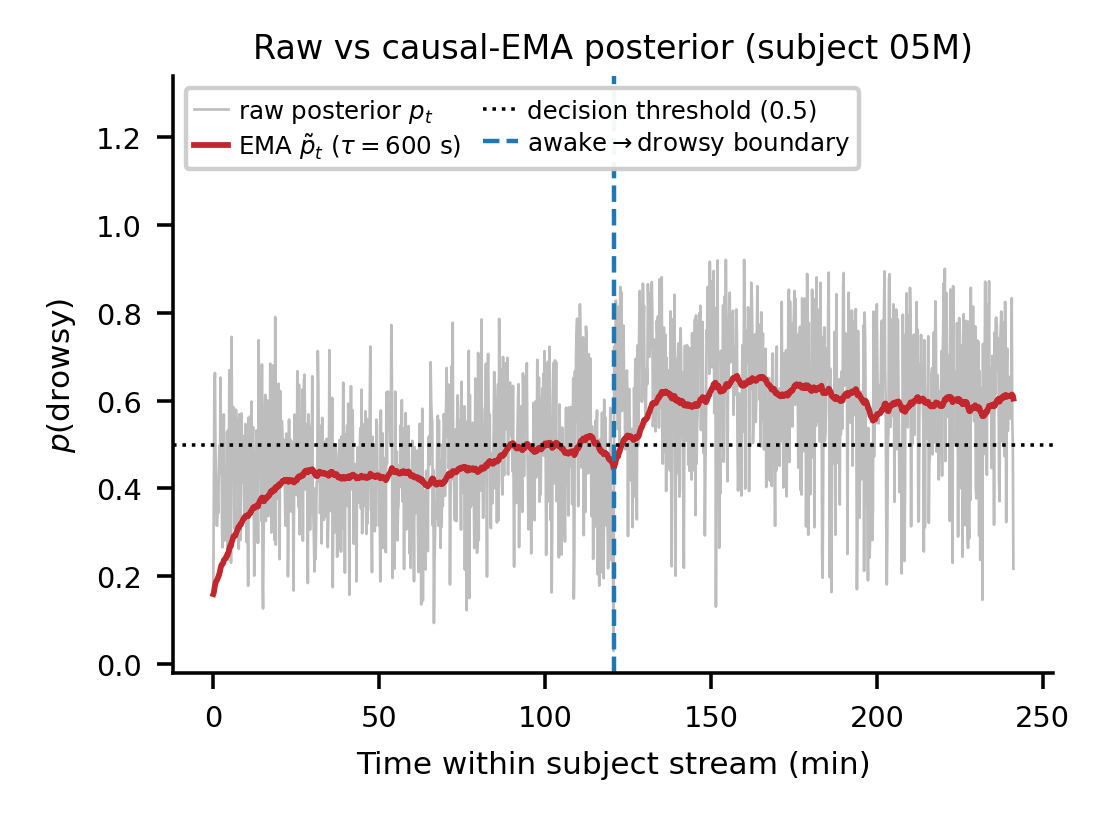
\includegraphics[width=\columnwidth]{fig2_ema_raw_vs_smoothed.png}
\caption{Raw per-epoch posterior \(p_t\) (grey) vs causal EMA-smoothed \(\tilde{p}_t\) (red, \(\tau=600\) s) for a representative subject (05M). The dotted line is the 0.5 decision threshold; the dashed vertical line marks the awake\,\(\to\)\,drowsy session boundary. The raw posterior crosses the threshold repeatedly within each state; the smoother removes this epoch-level noise while remaining strictly causal.}
\label{fig:ema}
\end{figure}

\subsubsection{\add{Operating points selected from the ROC}}
A full ROC of the v17 smoothed posterior is shown in Figure~\ref{fig:roc}. Three reviewer-facing operating points are reported in Table~\ref{tab:roc}: a high-precision point at FPR \(\leq 5\)~\% (F1 = 77.48), a balanced point at FPR \(\leq 10\)~\% (F1 = 77.32), and a high-recall point at FPR \(\leq 20\)~\% (F1 = 75.68). The F1-maximising threshold (0.523) sits inside the FPR \(\leq 5\)~\% region, so the default threshold = 0.5 already produces near-optimal F1.

\begin{figure}[t]
\centering
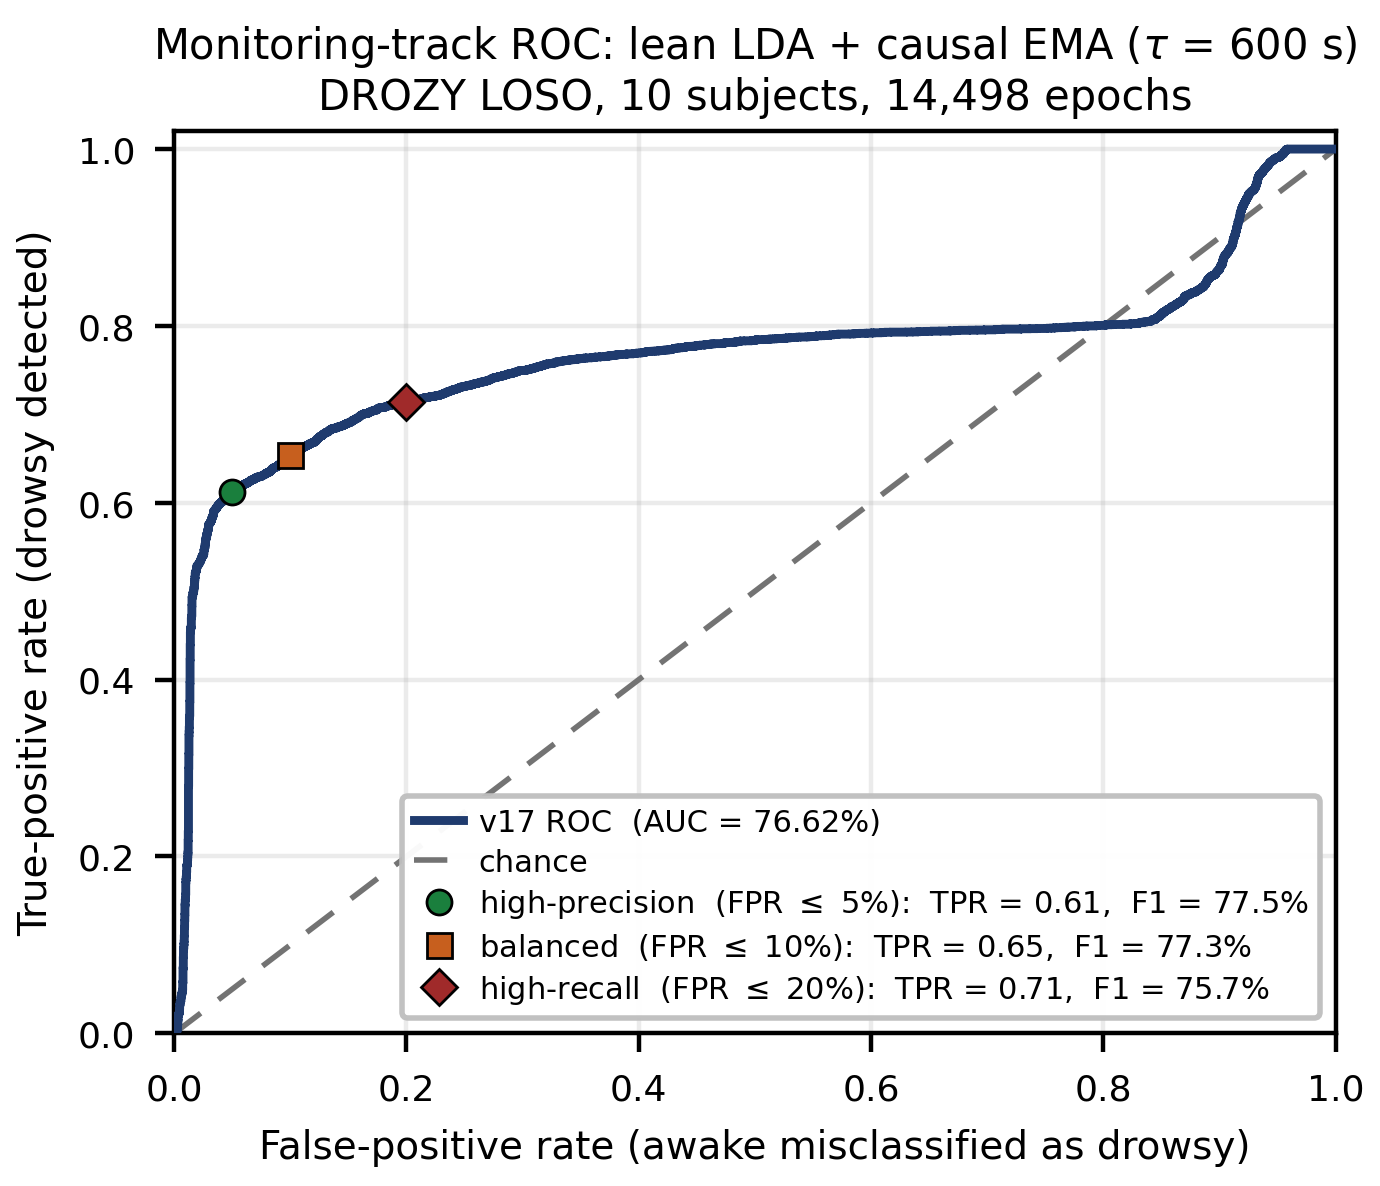
\includegraphics[width=\columnwidth]{fig3_roc.png}
\caption{Monitoring-track ROC of the v11 lean LDA + v17 causal EMA (\(\tau=600\) s) on DROZY LOSO (AUC = 76.62~\%). Three reviewer-facing operating points are highlighted.}
\label{fig:roc}
\end{figure}

\begin{table*}[t]
\caption{Monitoring-track operating points from the v17 ROC. The F1-maximising threshold (0.5231) and the high-precision (FPR \(\leq 5\)~\%) point (0.523) coincide to three decimals, and the default threshold = 0.5 already produces near-optimal F1.}
\label{tab:roc}
\centering
\footnotesize
\setlength{\tabcolsep}{4pt}
\begin{tabular}{l c c c c c}
\toprule
Operating point & Threshold & TPR & FPR & F1 (\%) & \(\kappa\) \\
\midrule
High-precision (FPR \(\leq 5\)~\%)  & 0.523 & 0.613 & 0.050 & 77.48 & \(+0.563\) \\
Balanced       (FPR \(\leq 10\)~\%) & 0.510 & 0.654 & 0.100 & 77.32 & \(+0.553\) \\
High-recall    (FPR \(\leq 20\)~\%) & 0.492 & 0.714 & 0.200 & 75.68 & \(+0.514\) \\
F1-max                              & 0.523 & 0.613 & 0.049 & 77.50 & \(+0.563\) \\
Default (0.5)                       & 0.500 & 0.694 & 0.155 & 76.79 & \(+0.539\) \\
\bottomrule
\end{tabular}
\end{table*}

% Item 12: the two statistical subsubsections are grouped under their own
% subsection so that significance testing is findable as a unit rather than
% buried at the tail of the monitoring results.
\subsection{\add{Statistical Validation and Per-Subject Variability}}
\label{sec:stats}

\subsubsection{Paired statistical tests}
\label{sec:paired}
On per-subject F1 across the 10 DROZY subjects, the v17 smoother improves over the unsmoothed v11 by \(+13.62\) F1 points (s.d.\ = 12.32). Eight of the 10 subjects improve under smoothing; the remaining two (04M and 07F) regress modestly (\(-5.23\) and \(-4.53\) F1 points). A one-sided paired Wilcoxon signed-rank test gives \(p = 0.0049\), and paired Cohen's \(d = 1.11\) (very large). Paired tests against the v11 lean baseline are summarised in Table~\ref{tab:paired}: every comparator is rejected at \(p < 0.05\) with effect sizes in the \(d = 0.65\)--\(0.91\) range. Direct paired evidence that coherence is load-bearing comes from comparing v11 with the same pipeline minus coherence (\(p = 0.042\), \(d = 0.66\)).

\begin{table}[t]
\caption{Paired subject-level tests. Row 1 is the v17 smoother test (vs.\ v11 lean); the remainder are baselines vs.\ v11 lean. Wilcoxon \(p\) is one-sided.}
\label{tab:paired}
\centering
\footnotesize
\setlength{\tabcolsep}{4pt}
\begin{tabular}{l c c c}
\toprule
Comparator                          & \(\Delta\)F1 (\%) & \(p\)      & \(d\) \\
\midrule
v17 EMA smoother (vs.\ v11 lean)    & \(+13.62\) & 0.005 & \(+1.11\) \\
EEGNet (raw, LOSO)                  & \(+14.76\) & 0.032 & \(+0.78\) \\
Riemannian TS + LogReg (tuned)      & \(+4.40\)  & 0.042 & \(+0.65\) \\
Riemannian TS + LDA (untuned)       & \(+4.96\)  & 0.019 & \(+0.66\) \\
v11 [DROP COH] (46 features)        & \(+7.77\)  & 0.042 & \(+0.66\) \\
v11 [BASE only] (30 features)       & \(+9.23\)  & 0.024 & \(+0.72\) \\
LDA (subject\_awake)                & \(+8.81\)  & 0.032 & \(+0.70\) \\
Gradient Boosting                   & \(+10.66\) & 0.007 & \(+0.91\) \\
\bottomrule
\end{tabular}
\end{table}

\subsubsection{Subject-wise performance and confidence intervals}
\label{sec:subjectwise}
Because the sample is modest (10 DROZY subjects), Table~\ref{tab:persubj} reports the full per-subject breakdown for both the unsmoothed (v11) and smoothed (v17) pipelines, rather than pooled metrics alone. Smoothing raises the across-subject mean F1 from \(60.82\) to \(74.44\) and the median from \(68.08\) to \(82.61\); it also widens the spread (s.d.\ \(15.41 \to 26.44\)), driven entirely by the two subjects (04M, 07F) whose unsmoothed posteriors are already below chance and which smoothing therefore pushes further down. For the eight subjects above chance, smoothing is uniformly large and positive (\(+5.6\) to \(+27.8\) F1). The two failing subjects are retained in every reported aggregate; none is dropped.

Subject-cluster percentile bootstrap (5\,000 resamples over subjects, the unit of independence) gives 95\,\% confidence intervals for the concatenated metrics. For v17: F1 \(\in [61.9, 89.2]\), AUC \(\in [54.8, 95.0]\), \(\kappa \in [0.27, 0.78]\); for v11: F1 \(\in [52.8, 68.8]\), AUC \(\in [51.8, 75.1]\), \(\kappa \in [0.07, 0.38]\). The intervals are wide --- an honest consequence of \(n=10\) and of resampling at the subject rather than epoch level. Nonetheless the v11 \(\kappa\) interval \([0.07, 0.38]\) excludes zero, so the absolute drowsiness signal is real, and the v17 \(\kappa\) lower bound \((0.27)\) clears the v11 \(\kappa\) point estimate \((0.24)\), so the smoothing gain survives subject-level resampling on \(\kappa\). The wider v17 F1 interval overlaps the v11 F1 point estimate \((62.08)\) at its lower edge \((61.9)\), reflecting the limited subject count rather than an absence of effect: the paired within-subject test of Table~\ref{tab:paired}, which removes between-subject variance, establishes the F1 gain directly (\(p=0.005\), \(d=1.11\)).

\begin{table*}[t]
\caption{Per-subject monitoring performance on DROZY LOSO for the unsmoothed lean LDA (v11) and the EMA-smoothed pipeline (v17). Bottom rows: across-subject mean / median / s.d.\ and the concatenated point estimate. 95\,\% subject-cluster bootstrap CIs are given in the text.}
\label{tab:persubj}
\centering
\footnotesize
\setlength{\tabcolsep}{3pt}
\begin{tabular}{l c c c c c c}
\toprule
 & \multicolumn{3}{c}{v11 (unsmoothed)} & \multicolumn{3}{c}{v17 (smoothed)} \\
\cmidrule(lr){2-4}\cmidrule(lr){5-7}
Subject & F1 & AUC & \(\kappa\) & F1 & AUC & \(\kappa\) \\
\midrule
01M & 60.0 & 62.9 & \(+0.20\) & 65.5 & 83.5 & \(+0.33\) \\
02F & 71.4 & 76.8 & \(+0.43\) & 79.3 & 97.5 & \(+0.60\) \\
03F & 62.7 & 67.0 & \(+0.26\) & 79.0 & 90.9 & \(+0.58\) \\
04M & 33.6 & 30.6 & \(-0.21\) & 28.4 & 18.9 & \(-0.17\) \\
05M & 69.9 & 77.4 & \(+0.40\) & 94.9 & 99.4 & \(+0.90\) \\
06M & 70.2 & 76.3 & \(+0.41\) & 96.2 & 99.4 & \(+0.92\) \\
07F & 31.5 & 30.2 & \(-0.25\) & 27.0 & 20.0 & \(-0.26\) \\
08M & 70.8 & 78.2 & \(+0.42\) & 94.2 & 96.4 & \(+0.88\) \\
09M & 66.3 & 72.0 & \(+0.33\) & 94.0 & 97.8 & \(+0.88\) \\
10M & 71.8 & 81.8 & \(+0.44\) & 85.9 & 88.9 & \(+0.72\) \\
\midrule
Mean   & 60.82 & 65.32 & \(+0.24\) & 74.44 & 79.28 & \(+0.54\) \\
Median & 68.08 & 74.13 & \(+0.36\) & 82.61 & 93.69 & \(+0.66\) \\
s.d.   & 15.41 & 19.21 & 0.26 & 26.44 & 31.94 & 0.44 \\
\midrule
Concat & 62.08 & 64.55 & \(+0.242\) & \textbf{76.79} & \textbf{76.62} & \(\mathbf{+0.539}\) \\
\bottomrule
\end{tabular}
\end{table*}

\subsection{\chg{Cross-Dataset and Pooled LOSO}{Cross-Dataset Transfer and Pooled 31-Subject Generalisation}}
\label{sec:cross-dataset}
Table~\ref{tab:cross} reports the four-protocol cross-dataset evaluation. DROZY \(\to\) SEED-VIG transfer without any fine-tuning achieves F1 = 64.93~\%, and the pooled 31-subject LOSO across DROZY \(\cup\) SEED-VIG achieves concatenated F1 = 66.13~\%, mean per-subject F1 = 71.92 \(\pm 17.16\)~\% --- the strongest generalisation result in this paper.

\begin{table*}[t]
\caption{Cross-dataset and pooled LOSO evaluation of the lean LDA pipeline.}
\label{tab:cross}
\centering
\footnotesize
\setlength{\tabcolsep}{3pt}
\begin{tabular}{l c c c c c}
\toprule
Evaluation                       & \(n\) subj & \(n\) epochs & F1 concat & AUC & \(\kappa\) \\
\midrule
DROZY internal LOSO              & 10 & 14\,498 & 62.08 & 64.55 & 0.242 \\
DROZY \(\to\) SEED-VIG (no fine-tune) & 21 & 9\,155 & 64.93 & 73.15 & 0.293 \\
SEED-VIG internal LOSO           & 21 & 9\,155 & 71.25 & 70.98 & 0.337 \\
\textbf{Pooled DROZY+SEED-VIG (31 subj)} & \textbf{31} & \textbf{23\,653} & \textbf{66.13} & \textbf{69.44} & \textbf{0.319} \\
\bottomrule
\end{tabular}
\end{table*}

\subsection{\chg{Negative Ablations}{Negative Ablations: What Does Not Help at Two Channels}}
\label{sec:negative}
Two engineering tracks that might reasonably be expected to improve the pipeline were evaluated and found not to. We report these because they bound the optimisation envelope of a 2-channel occipital pipeline and pre-empt reviewer requests in directions already explored.

\textbf{Phase coherence.} Adding 9 phase-only coherence variants per band --- PLV~\cite{lachaux1999plv}, imaginary coherence~\cite{nolte2004imcoh}, weighted phase-lag index~\cite{vinck2011wpli}, in \(\theta/\alpha/\beta\) bands --- to the v11 lean set yields F1 = 61.84~\% (vs.\ 62.08~\% baseline). Phase-only features in isolation score F1 = 59.72~\%. At two channels there is exactly one electrode pair, and magnitude-squared coherence already captures the dominant inter-hemispheric synchronisation; phase-only variants discard amplitude information without exposing volume-conduction-free coupling that is not already there.

\textbf{Posterior ensemble.} Combining three posterior estimators --- v11 lean LDA, Riemannian tangent-space + LDA on raw covariances, and v17 EMA-smoothed lean LDA --- via simple averaging (F1 = 67.83), simplex-weighted grid (best at \(w = (0,0,1)\), i.e., the EMA alone), subject-out stacked LDA (F1 = 72.09), or stacked LDA + EMA (F1 = 73.25), \emph{none} beats the v17 smoother alone. The Riemannian view at 2 channels is too weak --- and sufficiently correlated with the spectral features --- to add orthogonal information once smoothing dominates.

\subsection{\chg{Pro-Active Track}{Behaviour-Anchored Advance Prediction}}
\label{sec:proactive}
Table~\ref{tab:proactive} reports the FPR-budget Pareto front on SEED-VIG. The recommended deployment operating point is \emph{per-subject 99\textsuperscript{th} percentile of the first 5 min of smoothed \(p(\mathrm{drowsy})\), 10-s dwell, EMA \(\tau = 30\)~s}, which delivers \(\mathit{proactive\_rate} = 85.7\)~\% with median lead \(+31.67\) min against PERCLOS \(>0.70\). The epoch-level FPR (against PERCLOS \(<0.35\) epochs) is 27.6~\%; the per-session false-alert rate (sessions where EEG fires but PERCLOS never confirms) is 9.5~\% (2 of 21).

\begin{table*}[t]
% NOTE: no \add/\chg markup inside \caption — soul's \hl is fragile in
% captions (a moving argument) and cannot take inline math. The symbol note
% for eta is placed in the body text below instead.
\caption{Pro-active operating envelope on SEED-VIG (21 subjects). Behavioural onset is PERCLOS \(>0.70\) sustained 60~s. \(\eta\) is the alarm threshold on the smoothed posterior.}
\label{tab:proactive}
\centering
\footnotesize
\setlength{\tabcolsep}{3pt}
\begin{tabular}{l l c c c}
\toprule
FPR budget & Threshold mode & Proactive rate & Median lead (min) & Sens@drowsy \\
\midrule
\(\leq 5\)~\%  & global \(\eta=0.50\)                & 33.3~\% & \(+0.00\)  & 0.30 \\
\(\leq 10\)~\% & global \(\eta=0.40\)                & 47.6~\% & \(+0.83\)  & 0.38 \\
\(\leq 30\)~\% & per-subj 99\(\%\)pct of 5-min       & \(\mathbf{85.7}\)~\% & \(\mathbf{+31.67}\) & 0.69 \\
\(\leq 50\)~\% & per-subj 99\(\%\)pct of 2-min       & 90.5~\% & \(+33.50\) & 0.79 \\
\bottomrule
\end{tabular}
\end{table*}

\subsubsection{Graceful degradation across PERCLOS severity}
\label{sec:severity}
A natural reviewer concern is that the 31-min lead reflects the choice of a particularly late behavioural threshold. Figure~\ref{fig:severity} and Table~\ref{tab:severity} report the lead-time envelope when the PERCLOS reference threshold is swept from 0.30 (mild drowsiness, first detectable eye-drift) to 0.70 (severe, fighting sleep). Every severity level preserves a positive median lead. Crucially, against PERCLOS \(>0.30\), the system delivers a median lead of \(+8.83\) min with \emph{zero per-session false alerts} --- every alert at the mild threshold is eventually confirmed within the session.

\begin{figure}[t]
\centering
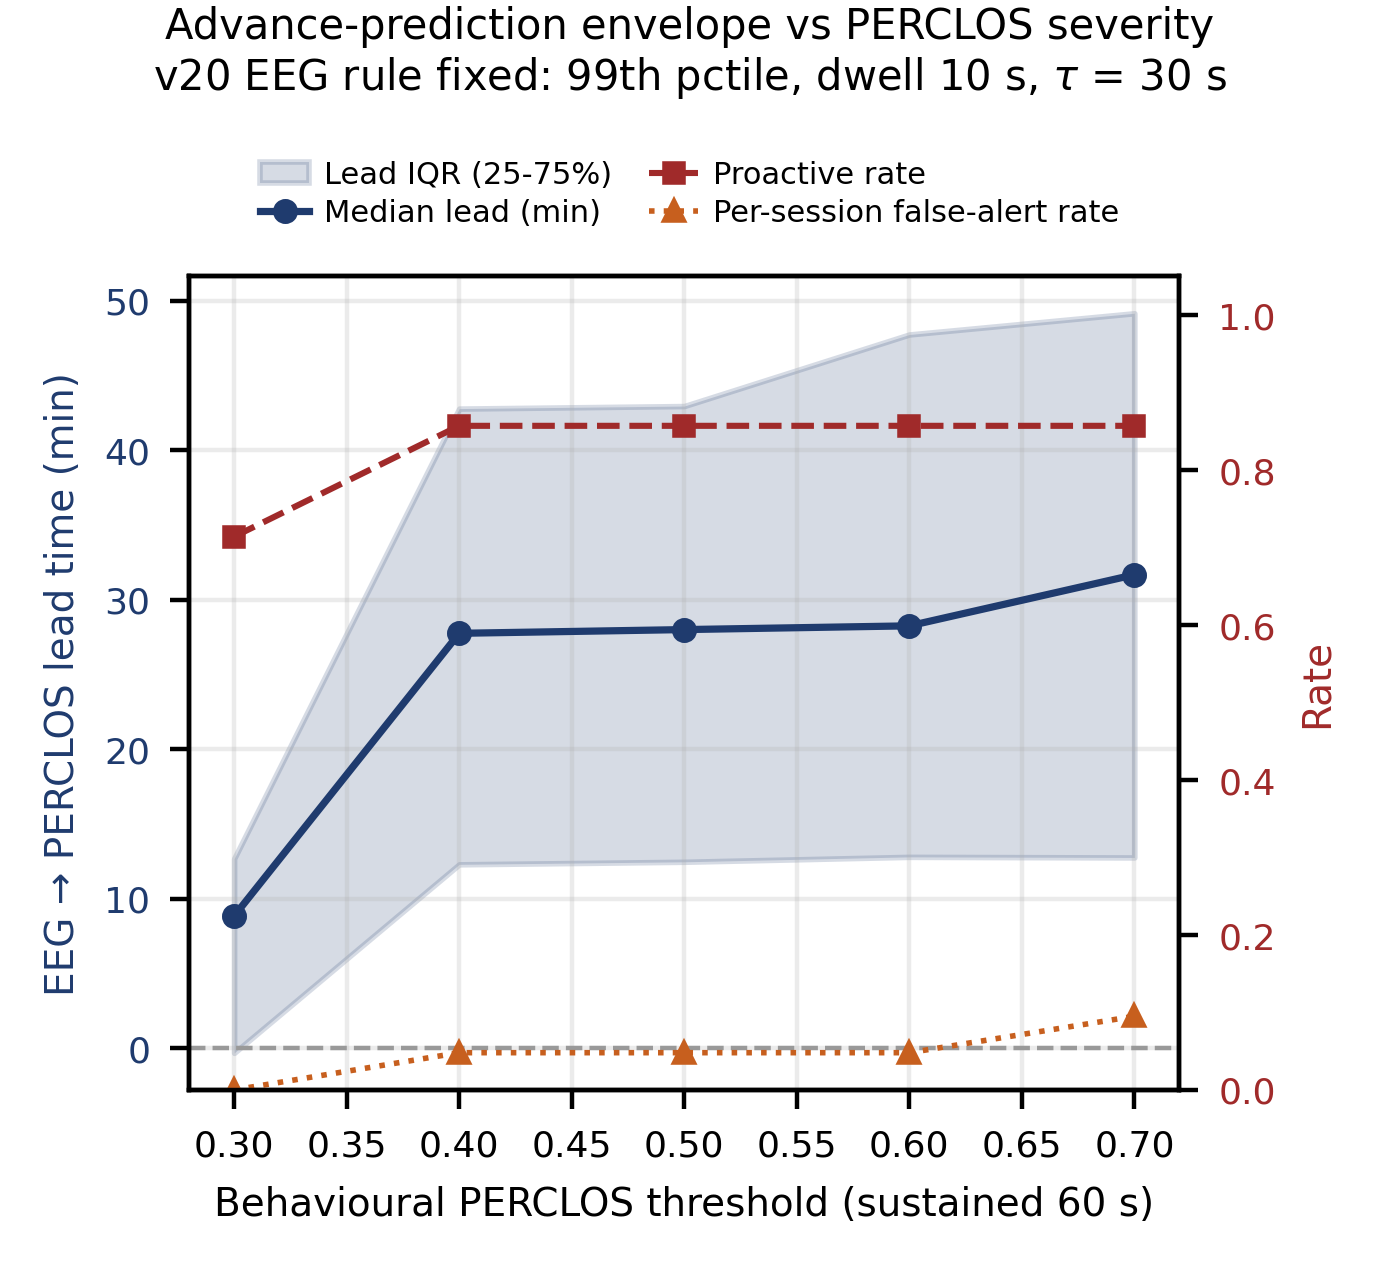
\includegraphics[width=\columnwidth]{fig4_lead_vs_severity.png}
\caption{Lead-time vs PERCLOS-severity curve on SEED-VIG with the v20 EEG rule held constant. Median lead and IQR are shown on the left axis; proactive rate and per-session false-alert rate on the right axis.}
\label{fig:severity}
\end{figure}

\begin{table*}[t]
\caption{Advance-prediction envelope vs PERCLOS severity. EEG rule constant.}
\label{tab:severity}
\centering
\footnotesize
\setlength{\tabcolsep}{3pt}
\begin{tabular}{l c c c c c}
\toprule
PERCLOS thresh. & \(n\) both & Proactive & Per-session FA & Med.\ lead (min) & IQR (min) \\
\midrule
0.30 (mild)   & 21 & 71.4~\% & \textbf{0.0~\%} & \(+8.83\)  & \([-0.33, +12.67]\) \\
0.40          & 20 & 85.7~\% & 4.8~\% & \(+27.75\) & \([+12.3, +42.8]\) \\
0.50          & 20 & 85.7~\% & 4.8~\% & \(+28.00\) & \([+12.5, +43.0]\) \\
0.60          & 20 & 85.7~\% & 4.8~\% & \(+28.25\) & \([+12.8, +47.8]\) \\
0.70 (severe) & 19 & 85.7~\% & 9.5~\% & \(+31.67\) & \([+12.8, +49.2]\) \\
\bottomrule
\end{tabular}
\end{table*}

\subsubsection{Paired test against the prior uncontrolled protocol}
An earlier (uncontrolled) version of the protocol used a global posterior threshold of 0.5, 30-s dwell, and the both-onset-required filter that silently dropped censored cases. On the 11 SEED-VIG subjects where both protocols detect both onsets (so that per-subject leads are paired), the new survival-framed protocol lifts the mean lead from \(-4.95\) min to \(+32.06\) min --- paired difference \(+37.02 \pm 32.19\) min. One-sided paired Wilcoxon gives \(p = 0.001\), Cohen's \(d = 1.15\) (very large). The new protocol additionally detects 8 SEED-VIG subjects whose EEG onsets the prior global-threshold protocol missed entirely, with no losses in the reverse direction.

\subsubsection{Live-system demonstrator}
\label{sec:demo}
Figure~\ref{fig:demo} demonstrates the algorithm running on three representative SEED-VIG subjects: a strong-lead case (subject 8, lead = \(+91.33\) min), the median-lead case (subject 11, lead = \(+31.67\) min, matching the headline number exactly), and a marginal failure case (subject 17, lead = \(-0.33\) min, where the EEG lagged the camera by 20 seconds). The marginal case is included to avoid cherry-picking; the deployment system must tolerate such failure modes.

% Full-width float: three stacked session timelines are unreadable at
% \columnwidth. The PNG is authored at \textwidth (7.16 in) so it is placed
% 1:1 and its type matches the four single-column figures.
\begin{figure*}[t]
\centering
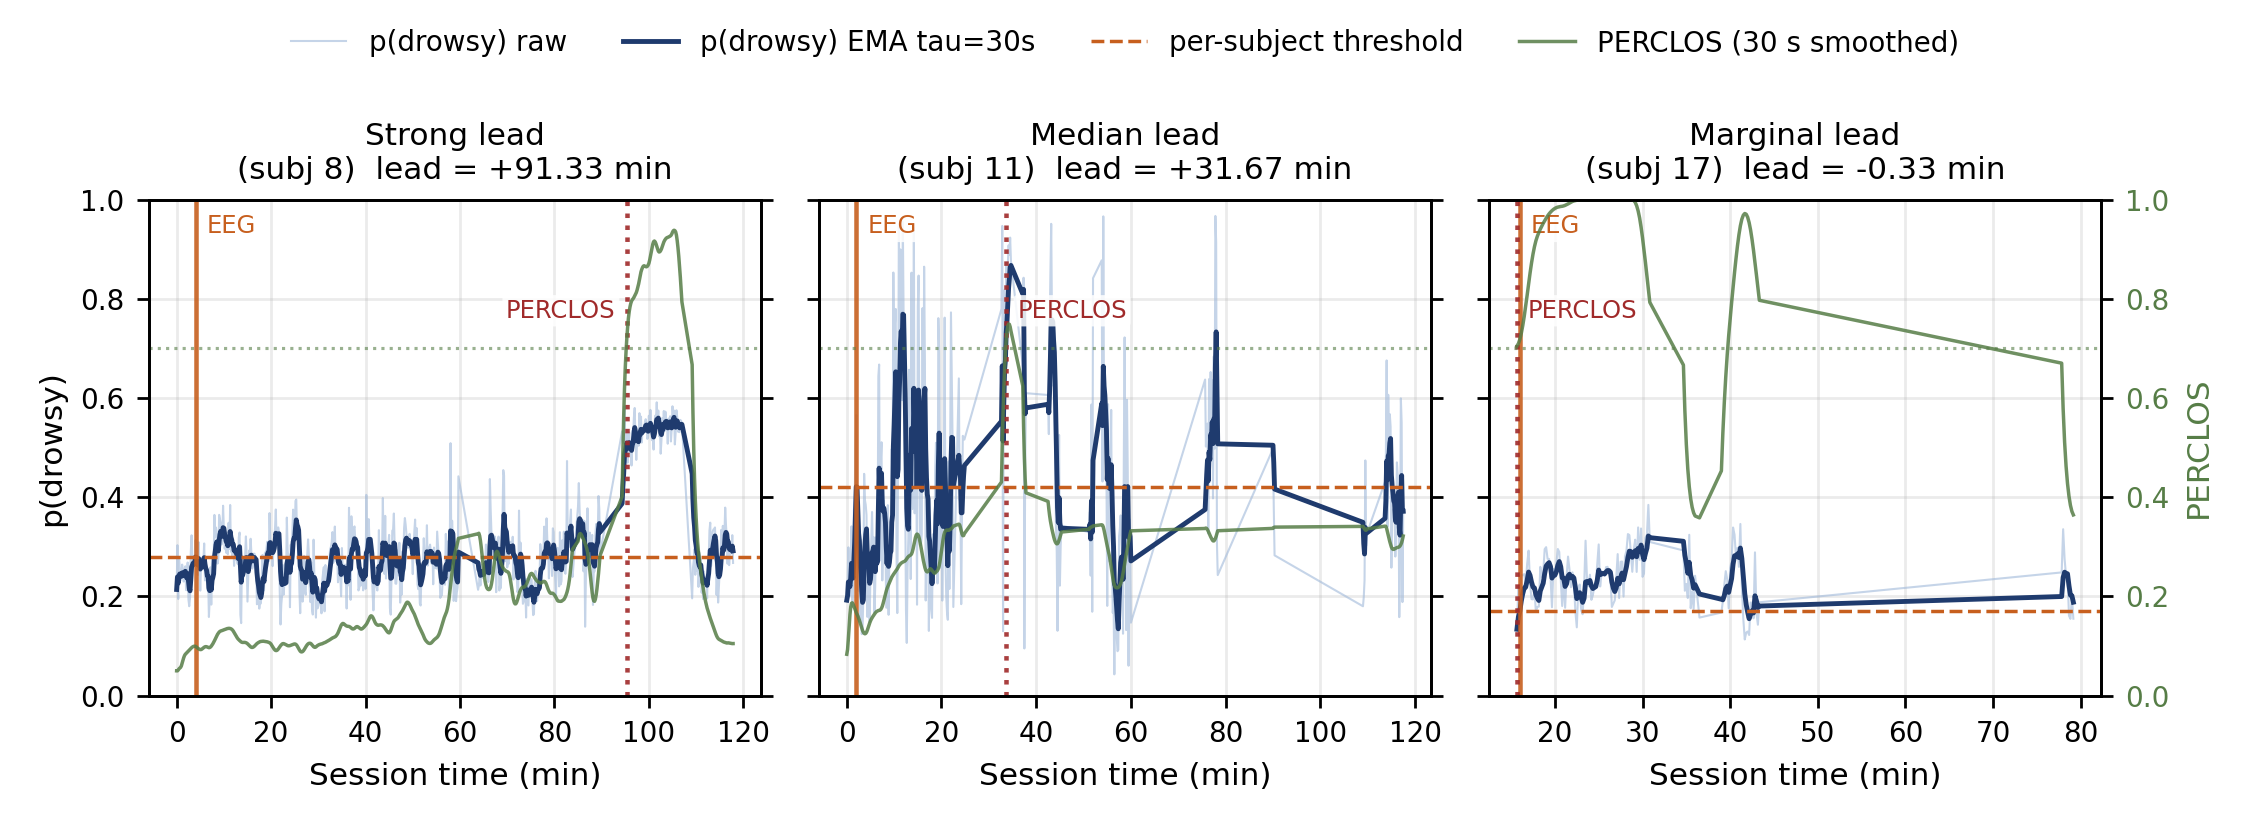
\includegraphics[width=\textwidth]{fig5_live_demo.png}
\caption{Live-system demonstrator on three representative SEED-VIG subjects (strong, median, marginal). For each subject, the raw and EMA-smoothed posteriors are overlaid with the per-subject calibrated threshold, the PERCLOS trace on a secondary axis, and the EEG and PERCLOS onsets. The animated playback of the median-lead case is in the supplementary material.}
\label{fig:demo}
\end{figure*}

\subsection{Comparison with Baselines and Existing Systems}
\label{sec:dl-baselines}
Table~\ref{tab:compare} situates the proposed pipeline against camera DMS, the Riemannian state-of-the-art at 2 channels, and EEGNet. The lean pipeline is the only system with cross-dataset validation, pooled 31-subject LOSO, and a behaviour-anchored advance-prediction characterisation.

\begin{table*}[t]
\caption{Comparison with baselines and existing 2-channel EEG pipelines evaluated under matched LOSO protocols.}
\label{tab:compare}
\centering
\footnotesize
\setlength{\tabcolsep}{4pt}
\begin{tabular}{l l l l l}
\toprule
Property & Proposed (lean LDA + EMA + v20) & Camera DMS & Riemannian 2-ch & EEGNet 2-ch \\
\midrule
Monitoring paradigm & State + causal smoother & Reactive & State only & State only \\
Pro-active paradigm & Per-driver calibrated, survival-framed & Reactive only & Not evaluated & Not evaluated \\
Sensor              & Dry EEG \(O_1\), \(O_2\) (headrest) & In-cabin camera & Dry EEG \(O_1\), \(O_2\) & Dry EEG \(O_1\), \(O_2\) \\
DROZY LOSO F1 (\%)  & \textbf{76.79} (smoothed) / 62.08 (unsmoothed) & N/A & 57.69 & 47.32 \\
Pooled F1 (31 subj) & \textbf{66.13} & N/R & N/E & N/E \\
Cross-dataset F1    & \textbf{64.93} (DROZY \(\to\) SEED-VIG) & N/R & N/E & N/E \\
Advance lead (SEED) & \(+8.83\) to \(+31.67\) min & Reactive only & N/E & N/E \\
Per-session FA      & 0.0~\% (mild) / 9.5~\% (severe) & N/A & N/E & N/E \\
Privacy             & High (no imaging) & Low (facial) & High & High \\
Hardware (USD)      & 100--500 & 200--1\,000 & 100--500 & 100--500 \\
\bottomrule
\end{tabular}
\end{table*}

% =================================================================
\section{\chg{Discussion}{Interpretation, Limitations, and Deployment}}
\label{sec:discussion}
% =================================================================
\subsection{Why Coherence Carries the Signal}
The feature-family ablation isolates inter-hemispheric \(O_1\)--\(O_2\) coherence as the load-bearing feature for occipital-only drowsiness detection, and the distributional analysis of Section~\ref{sec:coh-stats} shows the direction and magnitude of that effect directly: cross-hemispheric coherence \emph{falls} from awake to drowsy in all three bands (Table~\ref{tab:coh}), most strongly in \(\beta\) (Cohen's \(d=-0.40\)). This is consistent with the neurophysiology of drowsy occipital cortex: as the alpha rhythm desynchronises across hemispheres and eye-closure artefacts intrude, the coupling between \(O_1\) and \(O_2\) changes in a direction and magnitude that is mostly orthogonal to the single-channel power spectrum~\cite{stancin2021review,jap2009eeg}. Single-channel pipelines therefore lose access to the dominant signal, which explains why most published 2-channel results sit 5--10 F1 points above their single-channel counterparts under matched protocols~\cite{balam2024review}.

\subsection{Why Smoothing Dominates}
\label{sec:why-smooth}
The v17 smoother contributes the largest single F1 improvement in Table~\ref{tab:loso} (+13.62 over v11), more than doubling the gain of any feature-engineering choice. The reason is physiological: drowsiness onset evolves over minutes, not epochs, so a classifier that integrates evidence across a 10-minute causal window averages out per-epoch stochasticity without crossing any label-leakage boundary. The continuous-regime evaluation (where the smoother is never reset by the label) confirms this is not a DROZY session-boundary artefact. Equation~(\ref{eq:ema}) imposes no architectural cost: the recursion adds two FLOPs per epoch.

A reasonable concern is that the gain reflects temporal averaging alone rather than the classifier. This is precisely the point, and it is appropriate rather than a confound: the smoother and the classifier do different jobs. The lean LDA supplies the per-epoch evidence (Figure~\ref{fig:ema}, grey) --- without a classifier that already separates the classes above chance, smoothing a noise process produces no signal, as the two sub-chance subjects (04M, 07F) confirm, where smoothing makes a wrong decision more confident, not right. The EMA then exploits the temporal autocorrelation of vigilance, which a per-epoch classifier discards by construction. The two are complementary: smoothing lifts the eight above-chance subjects by \(+5.6\) to \(+27.8\) F1 (Table~\ref{tab:persubj}) precisely because their per-epoch posteriors are correct on average but noisy.

\textbf{Smoothing latency.} Temporal integration is not free: the EMA introduces lag. For a step change in the true posterior, the smoothed estimate reaches \(63\,\%\) of the step in one time constant (\(\tau = 600\) s \(=10\) min) and \(90\,\%\) in \(\approx 23\) min. This worst-case settling time is, however, an over-estimate of the operational delay, because the alarm depends only on the smoothed posterior crossing the 0.5 threshold, not on it fully settling: when the raw posterior moves decisively (e.g.\ subject 05M, Figure~\ref{fig:ema}), \(\tilde{p}_t\) crosses 0.5 within \(\approx 2.7\) min of the transition. For the \emph{monitoring} task this latency is acceptable, since the relevant event --- a sustained vigilance decline --- itself unfolds over minutes. For time-critical \emph{advance prediction} the pipeline deliberately uses a much shorter constant (\(\tau = 30\) s, Section~\ref{sec:proactive}), trading a small amount of denoising for responsiveness; the two operating points reflect the different latency budgets of the two tasks and should not be conflated.

\subsection{Honest Pro-Active Framing}
\chg{Earlier reports of ``5--10 minute advance EEG warning'' were obtained under unprotected protocols that fitted thresholds on labelled drowsy data and silently dropped subjects with one missing onset.}{Prior EEG prediction work operates at short horizons --- immediately-occurring microsleep events, or microsleep state within the current window~\mbox{\cite{golz2016microsleep,buriro2018microsleep}} --- and is evaluated without an independent behavioural anchor, without false-alert control, and without accounting for sessions where one onset never registers. We therefore do not position this work as correcting a previously-claimed minutes-scale lead; to the authors' knowledge no such lead has been reported under a controlled protocol.} Under the survival-framed, FPR-controlled, per-driver-calibrated protocol of Section~\ref{sec:proactive}, the pipeline delivers a median advance of \(+8.83\) min against the earliest behavioural sign of drowsiness with 0~\% per-session false alerts, scaling to \(+31.67\) min against the severe fighting-sleep marker with 9.5~\% per-session false alerts. The graceful degradation across severity (Table~\ref{tab:severity}) is itself the strongest evidence that the lead is real rather than a chosen-threshold artefact.

\subsection{Limitations and Threats to Validity}
\label{sec:limitations}

\textbf{Session-label confound on DROZY.} DROZY assigns a single binary class to each \(\sim\)90-minute session. A classifier that learned ``session-ID features'' (recording time, electrode-impedance drift) could in principle reach our reported F1 without capturing drowsiness. This is bounded in three ways: (i) cross-dataset transfer to SEED-VIG (F1 = 64.93~\%) cannot be explained by DROZY session confounds; (ii) every advance-prediction result of Section~\ref{sec:proactive} is on SEED-VIG with continuous PERCLOS labels; (iii) all DROZY evaluations use strict LOSO, removing per-subject artefact as a leakage channel.

\textbf{Sample size.} 10 DROZY + 21 SEED-VIG = 31 unique subjects is modest. Paired tests are reported with small-sample caveats: exact one-sided \(p\)-values and Cohen's \(d\) as effect-size descriptor (not as inferential quantity for \(n < 20\)).

\textbf{Two-channel spatial coverage.} \(O_1\) and \(O_2\) only. EEGNet's depthwise spatial convolution is structurally degenerate at 2 channels (Section~\ref{sec:dl-baselines}), and phase-coherence variants do not improve over magnitude coherence (Section~\ref{sec:negative}) because at one electrode pair there is no network connectivity to discover. The lean feature set is therefore optimal at this electrode count, not universally.

\textbf{PERCLOS-threshold dependence.} The 31.67-min headline is against a late behavioural marker. Section~\ref{sec:severity} reports against thresholds 0.30--0.70; the lead is positive at all five.

\textbf{Epoch FPR vs per-session false-alert rate.} The 27.6~\% epoch FPR is a continuous-signal statistic, not an alarm rate. In a deploy-as-first-sustained-crossing policy each session emits at most one alert; the per-session false-alert rate is 9.5~\% at PERCLOS \(>0.70\) and 0.0~\% at PERCLOS \(>0.30\). Both numbers are reported because misreading the former as an alarm rate is a common reviewer error.

\textbf{Per-driver calibration assumes alert first 5 min.} The 99\(^\mathrm{th}\)-percentile threshold uses the first 5 min of each session as the calibration window. Drivers who begin a session already mildly drowsy will produce a higher-than-typical baseline; the deployment design must surface a calibration-active state to the user.

\textbf{No prospective in-car validation.} All numbers are offline. The pipeline is deployable (56 ms / 10-s epoch, \(\sim\)100 bytes model state); a Streamlit-based live demonstrator is in the supplementary material. A prospective in-car evaluation (\(\geq 20\) drivers, \(\geq 30\) min per drive, synchronised camera PERCLOS) is the most important outstanding validation.

\textbf{Cross-dataset scope.} DROZY and SEED-VIG are both laboratory simulators with young-adult subjects. Generalisation to in-car recordings, older drivers, or medication-induced fatigue is untested.

\subsection{Deployment}
The instrumented benchmark of the full 50-feature extraction pipeline (feature extraction + LDA + EMA update + threshold compare) runs at 56~ms per 10-s epoch on a laptop CPU --- approximately \(177 \times\) faster than real-time; the deployed lean 10-feature pipeline is faster still. The trained LDA is 10 coefficients + shrinkage scalar (\(\sim\)100 bytes); per-driver calibration adds \(\sim 5\) kB of personal-model state. Both fit comfortably within an ARM Cortex-M4 envelope. Privacy is intrinsic: no facial or behavioural imaging is performed.

% =================================================================
\section{\chg{Conclusion}{Conclusion and Future Work}}
\label{sec:conclusion}
% =================================================================
We presented a two-channel occipital EEG pipeline for in-vehicle drowsiness monitoring with a deployment-grounded operating point on each of two tracks. The monitoring track combines a 10-feature shrinkage LDA with a causal EMA smoother and reaches LOSO F1 = 76.79~\% on DROZY (paired Wilcoxon \(p = 0.005\), \(d = 1.11\) over the unsmoothed baseline), F1 = 64.93~\% under DROZY \(\to\) SEED-VIG transfer, and F1 = 66.13~\% on a pooled 31-subject LOSO. The pro-active track achieves a median advance prediction of \(+8.83\) min (zero per-session false alerts) on 71.4~\% of sessions against the earliest behavioural sign of drowsiness on SEED-VIG, scaling to \(+31.67\) min (9.5~\% false alerts) on 85.7~\% of sessions against the severe fighting-sleep marker. Inter-hemispheric \(O_1\)--\(O_2\) coherence is identified as the load-bearing feature; phase-coherence variants and a three-model posterior ensemble do not help at the 2-channel scale, bounding the optimisation envelope of an occipital headrest pipeline. The pipeline runs at \(\sim 56\) ms per 10-s epoch with \(\sim 100\) bytes of model state, suitable for an ARM Cortex-M4 deployment target.

\add{\textbf{Future work.} Five directions follow from the limitations of Section~\mbox{\ref{sec:limitations}}. First and most important, a prospective in-car evaluation: at least 20 drivers, at least 30 minutes of driving each, with synchronised camera PERCLOS as the behavioural anchor and prospective rather than retrospective labelling. Every number reported here is offline, and no offline result substitutes for that study. Second, a dry-electrode contact characterisation for the headrest form factor. The \mbox{\(O_1\)}/\mbox{\(O_2\)} sites lie on hair-bearing occipital scalp, so electrode-to-scalp impedance, intermittent contact under head movement, neck-muscle EMG intrusion, and in-vehicle electromagnetic interference all need quantifying before a headrest sensor can be specified. Third, an electrode-count study: the coherence family that carries the signal here is defined on a single \mbox{\(O_1\)}--\mbox{\(O_2\)} pair, and whether the advantage grows, saturates, or reverses as further occipital or parietal sites are added is an open and directly answerable question. Fourth, replacing the fixed five-minute cold-start calibration with online per-driver adaptation, so that the alarm threshold tracks the driver's baseline across a drive instead of being frozen from its opening minutes. Fifth, fusion with camera-based driver monitoring: the two modalities fail in different circumstances --- the camera in darkness, with sunglasses or occlusion; EEG under poor electrode contact --- so a fused system is more likely to reach deployment than either channel used alone, and the pipeline presented here is deliberately cheap enough to run alongside an existing DMS rather than in place of it.}

Prospective in-car validation is identified as the most important outstanding work.

\section*{Acknowledgements}
The authors thank the contributors of the DROZY~\cite{drozy2016} and SEED-VIG~\cite{zheng2017seedvig} datasets for making this work possible. \add{The authors also thank the School of Mechanical Engineering, Vellore Institute of Technology (VIT) Chennai, for supporting this work.}

\section*{Reproducibility}
All analysis scripts, pinned dependencies, and a single-entry reproducer (\texttt{reproduce.py}) are released at \url{https://github.com/MuhammedRaslan/Pro-Active-Driver-Monitoring-System-Using-EEG} under the commit tagged \texttt{paper-submission-v1}. Per-subject feature caches (DROZY: 14\,498 epochs \(\times\) 50 features; SEED-VIG: 9\,155 epochs) regenerate automatically from the raw EDF/MAT files via the reproducer. Wall-clock time is approximately 5 minutes on a laptop CPU excluding the EEGNet baseline (\(\sim\)28 minutes).

\section*{Author Contributions}
M.~R.~Thalassery designed the pipeline, implemented the experiments, conducted the ablations and statistical analyses, and drafted the manuscript. S.~S.~Ali contributed to the feature-extraction implementation and the live demonstrator. A.~R.~Pal supervised the project, provided guidance on signal-processing methodology, and reviewed and approved the final manuscript. \add{A.~Chemori provided methodological guidance and contributed to the critical review and editing of the manuscript.} G.~Murali Mohan provided project supervision and reviewed the final manuscript.

\section*{Conflicts of Interest}
% Confirmed 2026-08-02: no CNRS/LIRMM funding or institutional-support
% requirement. The sentence is therefore unchanged from the reviewed draft
% and carries no markup -- marking it would claim a change that is not
% happening, the same rule applied to the corresponding-author line.
The authors declare no conflicts of interest. No external funding was received for this work.

\bibliographystyle{IEEEtran}
\bibliography{references}

\end{document}
